
\documentclass[a4paper,11pt]{article}
\usepackage{amsmath,amsthm,amsfonts,amssymb,amscd,amstext,vmargin,graphics,graphicx,tabularx,multicol} 
\usepackage[francais]{babel}
\usepackage[utf8]{inputenc}  
\usepackage[T1]{fontenc} 
\usepackage{pstricks-add,tikz,tkz-tab,variations}
\usepackage[autolanguage,np]{numprint} 

\setmarginsrb{1.5cm}{0.5cm}{1cm}{0.5cm}{0cm}{0cm}{0cm}{0cm} %Gauche, haut, droite, haut
\newcounter{numexo}
\newcommand{\exo}[1]{\stepcounter{numexo}\noindent{\bf Exercice~\thenumexo} : \marginpar{\hfill /#1}}
\reversemarginpar


\newcounter{enumtabi}
\newcounter{enumtaba}
\newcommand{\q}{\stepcounter{enumtabi} \theenumtabi.  }
\newcommand{\qa}{\stepcounter{enumtaba} (\alph{enumtaba}) }
\newcommand{\initq}{\setcounter{enumtabi}{0}}
\newcommand{\initqa}{\setcounter{enumtaba}{0}}

\newcommand{\be}{\begin{enumerate}}
\newcommand{\ee}{\end{enumerate}}
\newcommand{\bi}{\begin{itemize}}
\newcommand{\ei}{\end{itemize}}
\newcommand{\bp}{\begin{pspicture*}}
\newcommand{\ep}{\end{pspicture*}}
\newcommand{\bt}{\begin{tabular}}
\newcommand{\et}{\end{tabular}}
\renewcommand{\tabularxcolumn}[1]{>{\centering}m{#1}} %(colonne m{} centrée, au lieu de p par défault) 
\newcommand{\tnl}{\tabularnewline}

\newcommand{\bmul}[1]{\begin{multicols}{#1}}
\newcommand{\emul}{\end{multicols}}

\newcommand{\trait}{\noindent \rule{\linewidth}{0.2mm}}
\newcommand{\hs}[1]{\hspace{#1}}
\newcommand{\vs}[1]{\vspace{#1}}

\newcommand{\N}{\mathbb{N}}
\newcommand{\Z}{\mathbb{Z}}
\newcommand{\R}{\mathbb{R}}
\newcommand{\C}{\mathbb{C}}
\newcommand{\Dcal}{\mathcal{D}}
\newcommand{\Ccal}{\mathcal{C}}
\newcommand{\mc}{\mathcal}

\newcommand{\vect}[1]{\overrightarrow{#1}}
\newcommand{\ds}{\displaystyle}
\newcommand{\eq}{\quad \Leftrightarrow \quad}
\newcommand{\vecti}{\vec{\imath}}
\newcommand{\vectj}{\vec{\jmath}}
\newcommand{\Oij}{(O;\vec{\imath}, \vec{\jmath})}
\newcommand{\OIJ}{(O;I,J)}


\newcommand{\reponse}[1][1]{%
\multido{}{#1}{\makebox[\linewidth]{\rule[0pt]{0pt}{20pt}\dotfill}
}}

\newcommand{\titre}[5] 
% #1: titre #2: haut gauche #3: bas gauche #4: haut droite #5: bas droite
{
\noindent #2 \hfill #4 \\
#3 \hfill #5

\vspace{-1.6cm}

\begin{center}\rule{6cm}{0.5mm}\end{center}
\vspace{0.2cm}
\begin{center}{\large{\textbf{#1}}}\end{center}
\begin{center}\rule{6cm}{0.5mm}\end{center}
}



\begin{document}
\pagestyle{empty}
\titre{Contrôle - Le théorème de Pythagore et sa réciproque}{Nom :}{Prénom :}{Classe}{Date}


\vspace*{0.3cm}

\exo{4} Entourer \textbf{la ou les} bonnes réponses.
\renewcommand{\arraystretch}{2}
\vspace*{0.3cm}

\begin{tabular}{|p{6cm}|c|c|c|}
\hline 
 & \textbf{REPONSE A} & \textbf{REPONSE B} & \textbf{ REPONSE C} \\ 
\hline 
\textbf{Si le triangle GSD est rectangle en S alors ...} & $GS^{2}=GD^{2}+DS^{2}$ & $GD^{2}=GS^{2}+SD^{2}$ & $SD^{2}=SG^{2}+GD^{2}$ \\ 
\hline 
$\sqrt{196}= ...$ & 14 & -14 & 98 \\ 
\hline 
\textbf{Si $AZ^{2}=AU^{2}+UZ^{2}$ alors le triangle AUZ est rectangle en ...} & A & U & Z \\ 
\hline 
\textbf{Le triangle ABC est rectangle en B tel que AB = 333 cm et BC = 444  cm. La longueur AC vaut ... } & 777 & 666 & 555 \\ 
\hline 
\end{tabular} 

\vspace*{0.7cm}

\exo{3}  Donner une valeur approchée, au dixième près, de la longueur LM.
\begin{center}
\includegraphics[scale=0.65]{exothm2.eps} 
\end{center}


\exo{3} Le triangle ABC est-il rectangle ?

\begin{center}

\includegraphics[scale=1.7]{recipythagore.eps} 
\end{center}



\exo{4} 

\bmul{2}
On a fixé au mur une étagère [ET] en la soutenant par un support [SP].\\
ST = 17,6 cm TP = 33 cm SP = 37,4 cm.\\
On suppose que le mur est vertical.\\
\vspace*{0.5cm}
L'étagère est-elle horizontale ?\\

\columnbreak

\includegraphics[scale=0.8]{reciproquepythagore.eps} \\

\emul

\newpage
\vspace*{0.7cm}

\exo{6} 
\bmul{2}
Une échelle appuyée contre un mur vertical se trouve à 5 m du mur. (la figure n'est pas à l'échelle) Elle glisse le long du mur de 80 cm.\\
 Elle se trouve à 11,2 m du sol et s'est éloignée d'une longueur de $x$ en m sur le sol.\\
 
$\rightarrow$ \textbf{Calculer la longueur $x$.}\\

\textit{Toute trace de recherche, même incomplète, ou d'initiative même infructueuse, sera prise en compte dans l'évaluation.}\\

\columnbreak

\includegraphics[scale=1.4]{exothm1.eps} \\

\emul





\end{document}
